% Define block styles
\tikzstyle{block} = [rectangle, fill=white, text centered, rounded corners]
\tikzstyle{arrow} = [draw]
\usetikzlibrary{matrix}

\pgfdeclareimage[width=11em]{ImBlock}{./figures/sec/secexample_blocksmarkednumbered.jpg}
\pgfdeclareimage[width=11em]{ImGraph}{./figures/sec/secexample_graph.png}

\definecolor{red1}{RGB}{160,0,0}
\definecolor{green1}{RGB}{0,160,0}
\definecolor{blue1}{RGB}{0,0,160}

	      
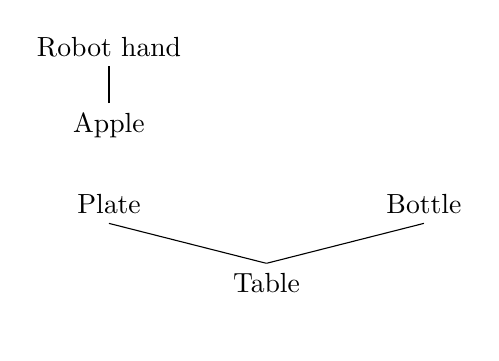
\begin{tikzpicture}[node distance=1cm, auto]
    \node[block] (table) {Table};
    \node[block, above of=table, xshift=-2cm, color=white] (appleW) {Robot hand};

    \node[block, above of=table, xshift=2cm] (bottle) {Bottle};
    \node[block, above of=table, xshift=-2cm] (plate) {Plate};
    \node[block, above of=plate] (apple) {Apple};
    \node[block, above of=apple] (hand) {Robot hand};

    % lines
    \draw [arrow] (table.north) to (plate.south);
    \draw [arrow] (table.north) to (bottle.south);
    \draw [arrow] (apple.north) to (hand.south);

    % alignment
    \node[block, below of=table, color=white, node distance=0.4cm] (appleW) {Robot hand};
    \node[block] (table) {Table};
\end{tikzpicture}
